% !TEX TS-program = pdflatex
% !TEX encoding = UTF-8 Unicode

% This file is a template using the "beamer" package to create slides for a talk or presentation
% - Talk at a conference/colloquium.
% - Talk length is about 20min.
% - Style is ornate.

% MODIFIED by Jonathan Kew, 2008-07-06
% The header comments and encoding in this file were modified for inclusion with TeXworks.
% The content is otherwise unchanged from the original distributed with the beamer package.


\documentclass{beamer}

% No navigation symbols in bottom right corner
\beamertemplatenavigationsymbolsempty

% Quote environment with author
\def\signed #1{{\leavevmode\unskip\nobreak\hfil\penalty50\hskip2em
  \hbox{}\nobreak\hfil(#1)%
  \parfillskip=0pt \finalhyphendemerits=0 \endgraf}}

\newsavebox\mybox
\newenvironment{aquote}[1]
  {\savebox\mybox{#1}\begin{quote}}
  {\signed{\usebox\mybox}\end{quote}}

\mode<presentation>
{
  \usetheme{Warsaw}
  % or ...

  \setbeamercovered{transparent}
  % or whatever (possibly just delete it)
}

\addtobeamertemplate{navigation symbols}{}{%
    \usebeamerfont{footline}%
    \usebeamercolor[fg]{footline}%
    \hspace{1em}%
    \insertframenumber
}
\setbeamercolor{footline}{fg=blue}

% Color for fonts
\usepackage{xcolor}

\usepackage[english]{babel}
% or whatever

\usepackage[utf8]{inputenc}
% or whatever

\usepackage{times}
\usepackage[T1]{fontenc}
% Or whatever. Note that the encoding and the font should match. If T1
% does not look nice, try deleting the line with the fontenc.


\title[ID2205 Final Presentation] % (optional, use only with long paper titles)
{A Development Environment for Decomposite MAC Description Language}
\subtitle{Final Presentation}

\author{Leon Fernandez}

\date{KTH Kista, Jan 2019}
% - Either use conference name or its abbreviation.
% - Not really informative to the audience, more for people (including
%   yourself) who are reading the slides online

\subject{}
% This is only inserted into the PDF information catalog. Can be left
% out. 



% If you have a file called "university-logo-filename.xxx", where xxx
% is a graphic format that can be processed by latex or pdflatex,
% resp., then you can add a logo as follows:

% \pgfdeclareimage[height=0.5cm]{university-logo}{university-logo-filename}
% \logo{\pgfuseimage{university-logo}}



\begin{document}

\begin{frame}
 	\titlepage
\end{frame}

\begin{frame}{Outline}
	\tableofcontents[hideallsubsections]
\end{frame}

%\section{ID2205}
%\subsection{Brief Description}
%\begin{frame}{Brief Description}
%\begin{aquote}{KTH Course web}
%	''After this course, the student will be able to plan and execute a design,
%	implementation, research, or equivalent task in software systems and report its outcomes.''
%\end{aquote}
%\end{frame}

%\subsection{Goals}
%\begin{frame}{Goals}
%	\begin{itemize}
%		\item Learning Outcomes
%		\begin{itemize}
%			\item Medium Access Control (MAC) protocols
%			\item Web development
%			\item User Interface (UI) design
%		\end{itemize}
%
%		\item Deliverables
%		\begin{itemize}
%			\item Simple web-based Development Environment (DE)
%			\item Syntax check
%			\item (Optional) Export to platform-independent format (.xml) 
%		\end{itemize}
%	\end{itemize}
%\end{frame}

\section{Background}
\subsection{Software Defined Radios}
\begin{frame}{Software Defined Radios}
	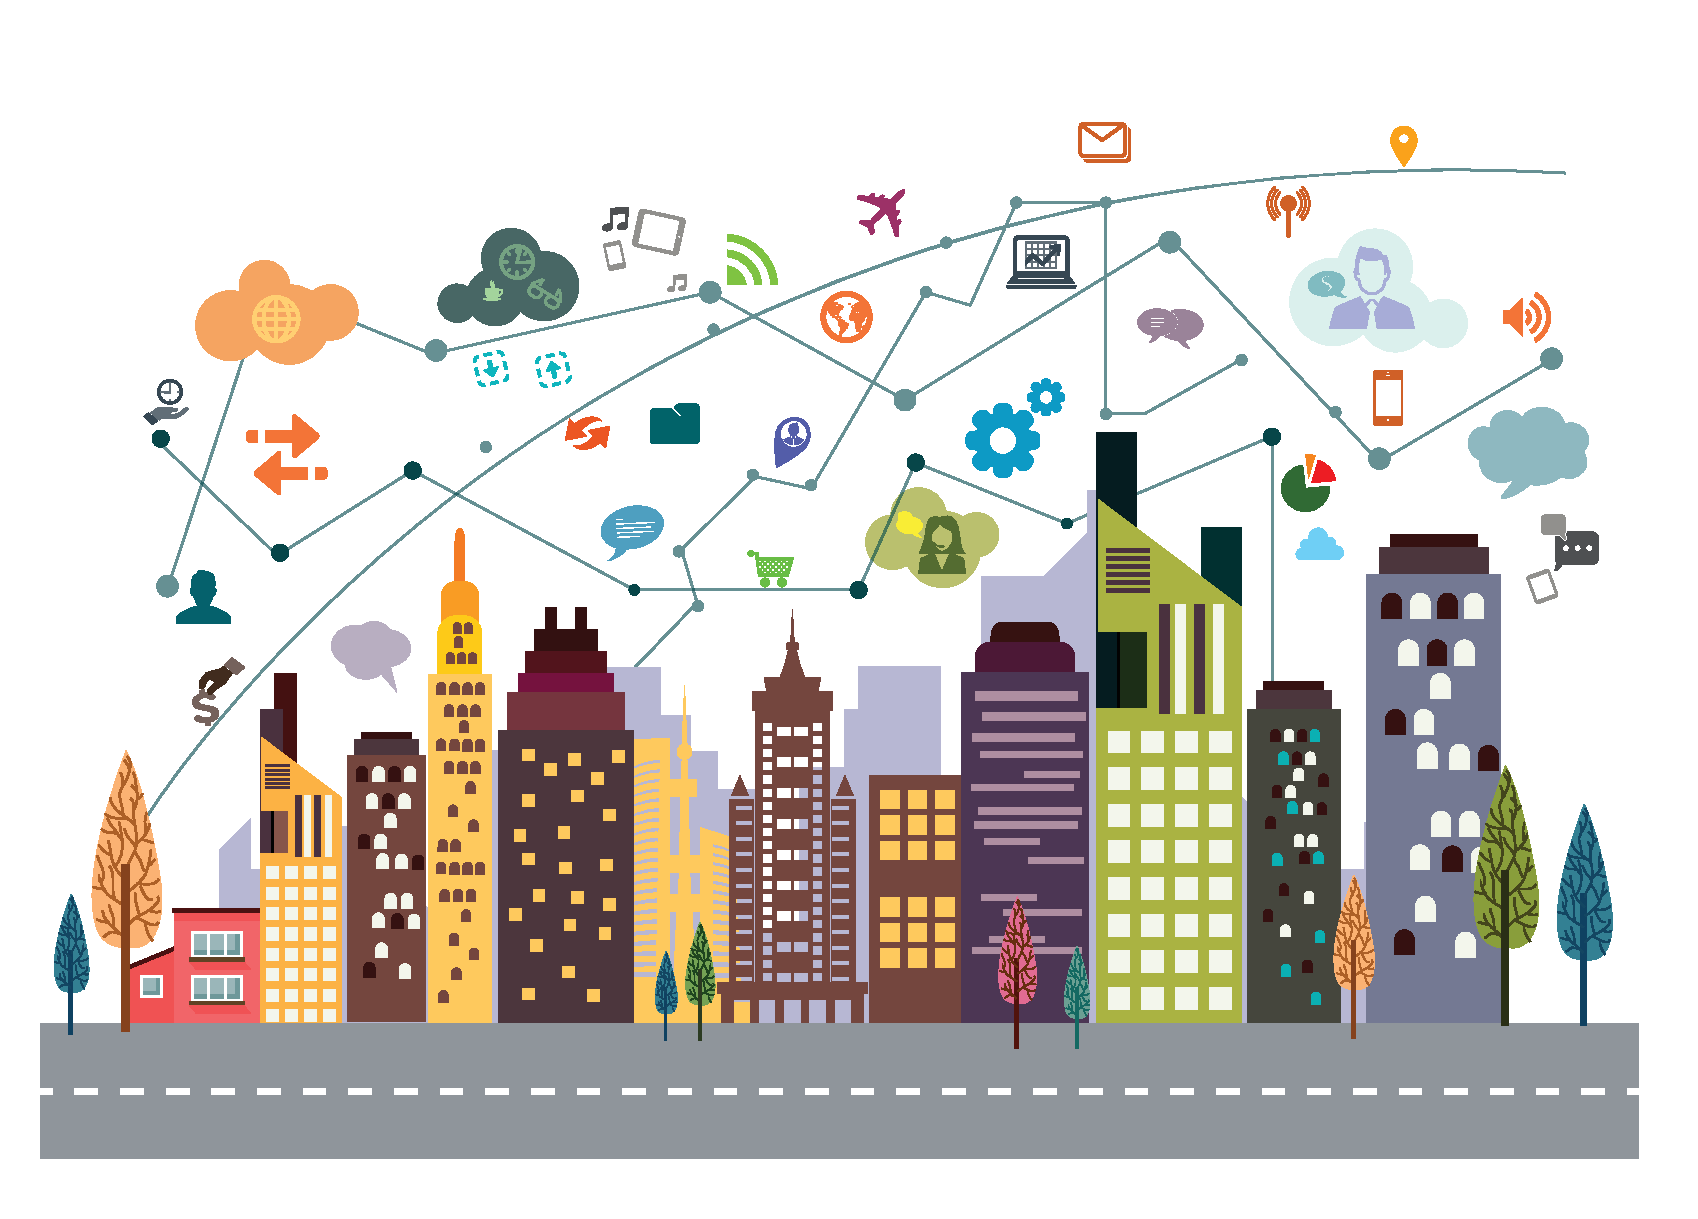
\includegraphics[width=\linewidth]{digital.eps}
	%https://all-free-download.com/free-vector/download/digital-communication-concept-cityscape-and-ui-design-style_6826344.html
\end{frame}
\begin{frame}{Software Defined Radios}
	\begin{figure}
 		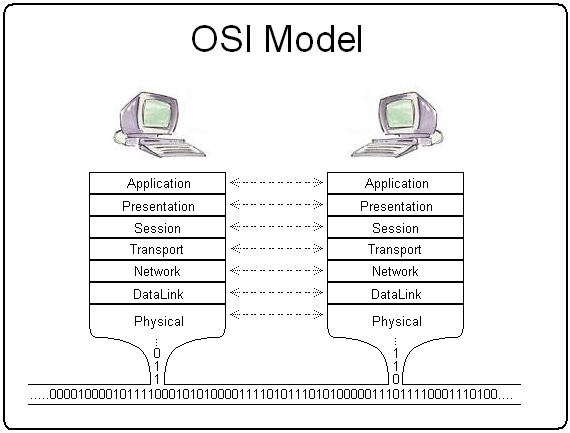
\includegraphics[width=0.65\linewidth]{osi.jpg}
 		\label{fig:osi}
	\end{figure}
\end{frame}

\subsection{Medium Access Control}
\begin{frame}{Medium Access Control}
	
\includegraphics[width=0.2\linewidth]{wireless.eps}
	\hfill
	
\includegraphics[width=0.2\linewidth]{wireless.eps}
\end{frame}

\begin{frame}{Medium Access Control}
	
\includegraphics[width=0.2\linewidth]{wireless.eps}
	\hfill
	
\includegraphics[width=0.2\linewidth]{wave.eps}
	
\includegraphics[width=0.2\linewidth]{wireless.eps}
\end{frame}

\begin{frame}{Medium Access Control}
	
\includegraphics[width=0.2\linewidth]{wireless.eps}
	
\includegraphics[width=0.2\linewidth,angle=180,origin=c]{wave.eps}
	\hfill
	
\includegraphics[width=0.2\linewidth]{wireless.eps}
\end{frame}

\begin{frame}{Medium Access Control}
	
\includegraphics[width=0.2\linewidth]{wireless.eps}
	
\includegraphics[width=0.2\linewidth,angle=180,origin=c]{wave.eps}
	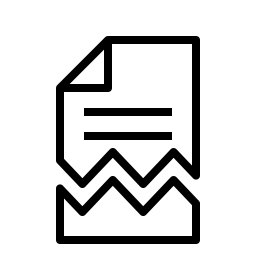
\includegraphics[width=0.16\linewidth]{error.png}
	%https://www.iconfinder.com/photo3idea
	
\includegraphics[width=0.2\linewidth]{wave.eps}
	
\includegraphics[width=0.2\linewidth]{wireless.eps}
\end{frame}

\begin{frame}{Decomposite MAC Description Language}
    Dmdl uses HFSM, that is better than traditional EFSM. (Elaborate)
\end{frame}

\begin{frame}{Decomposite MAC Description Language}
	\begin{figure}
 		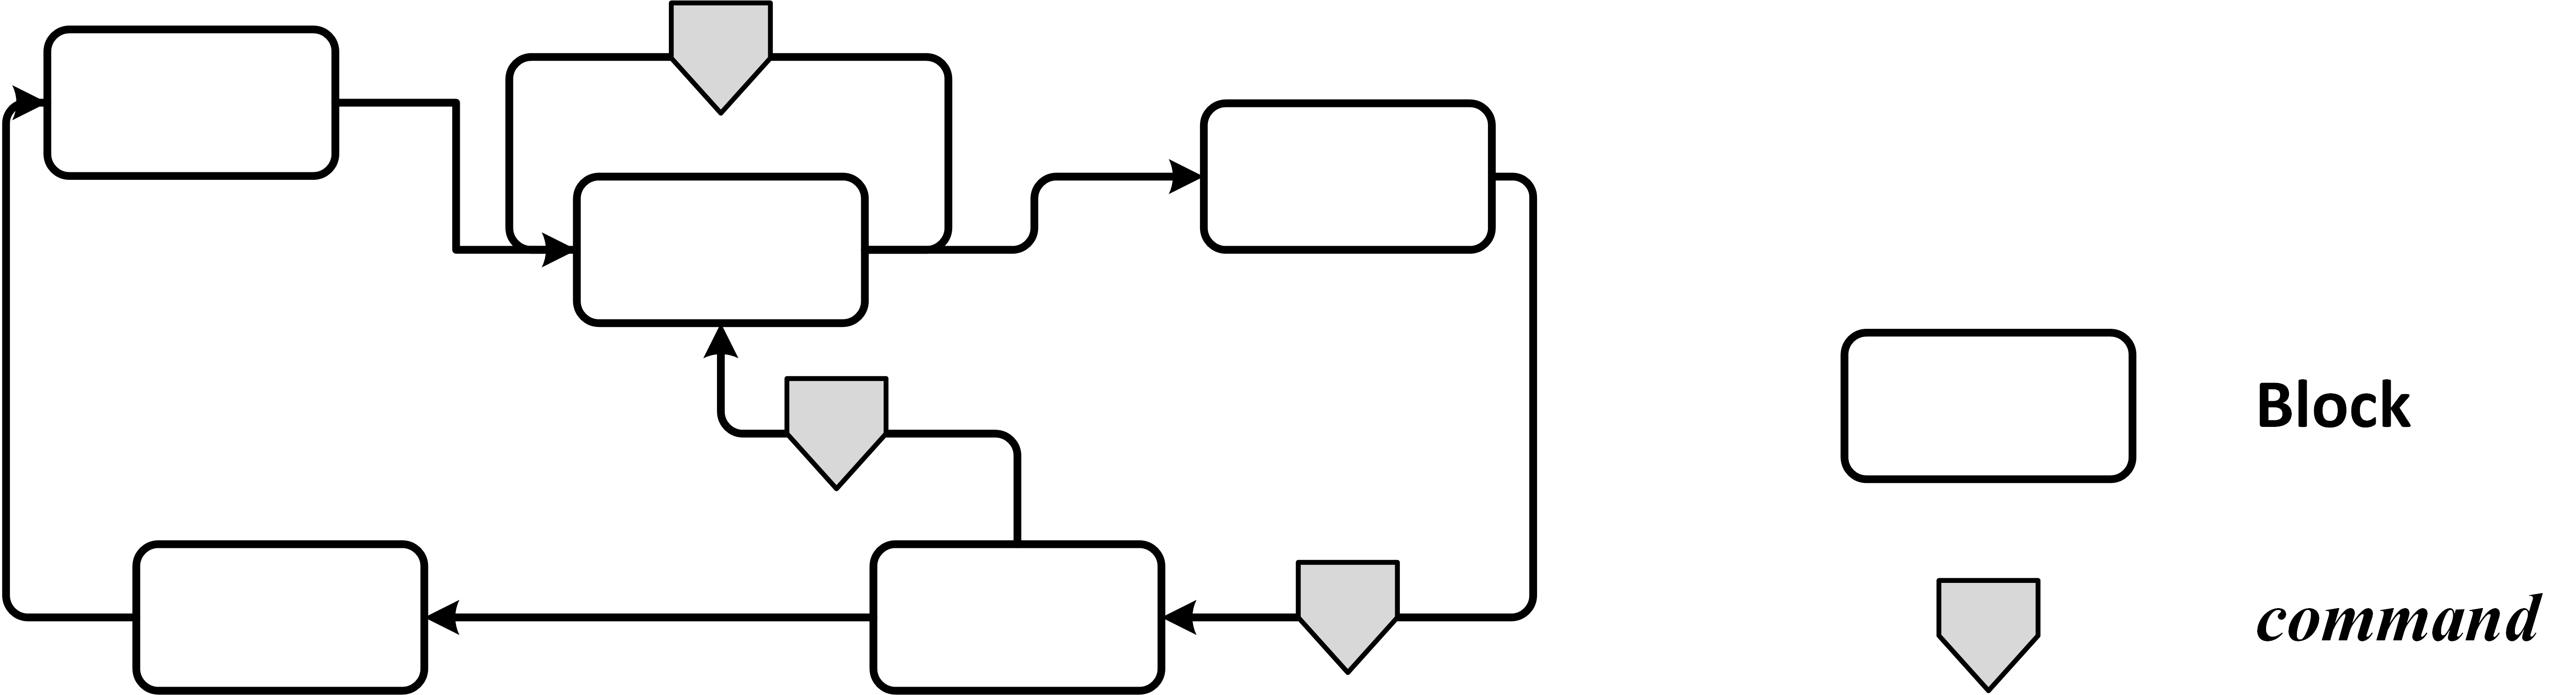
\includegraphics[width=\linewidth]{graph.png}
 		\label{fig:graph}
	\end{figure}
\end{frame}

\subsection{Decomposite MAC Description Language}
\begin{frame}{Decomposite MAC Description Language}
	\begin{figure}
 		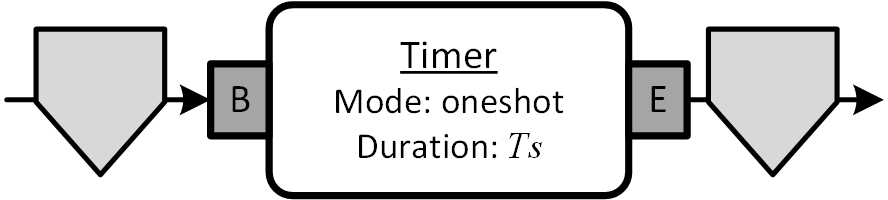
\includegraphics[width=\linewidth]{simple_timer.png}
 		\label{fig:timer}
	\end{figure}
\end{frame}

\subsection{Motivation}
\begin{frame}{Motivation}
	\begin{figure}
 		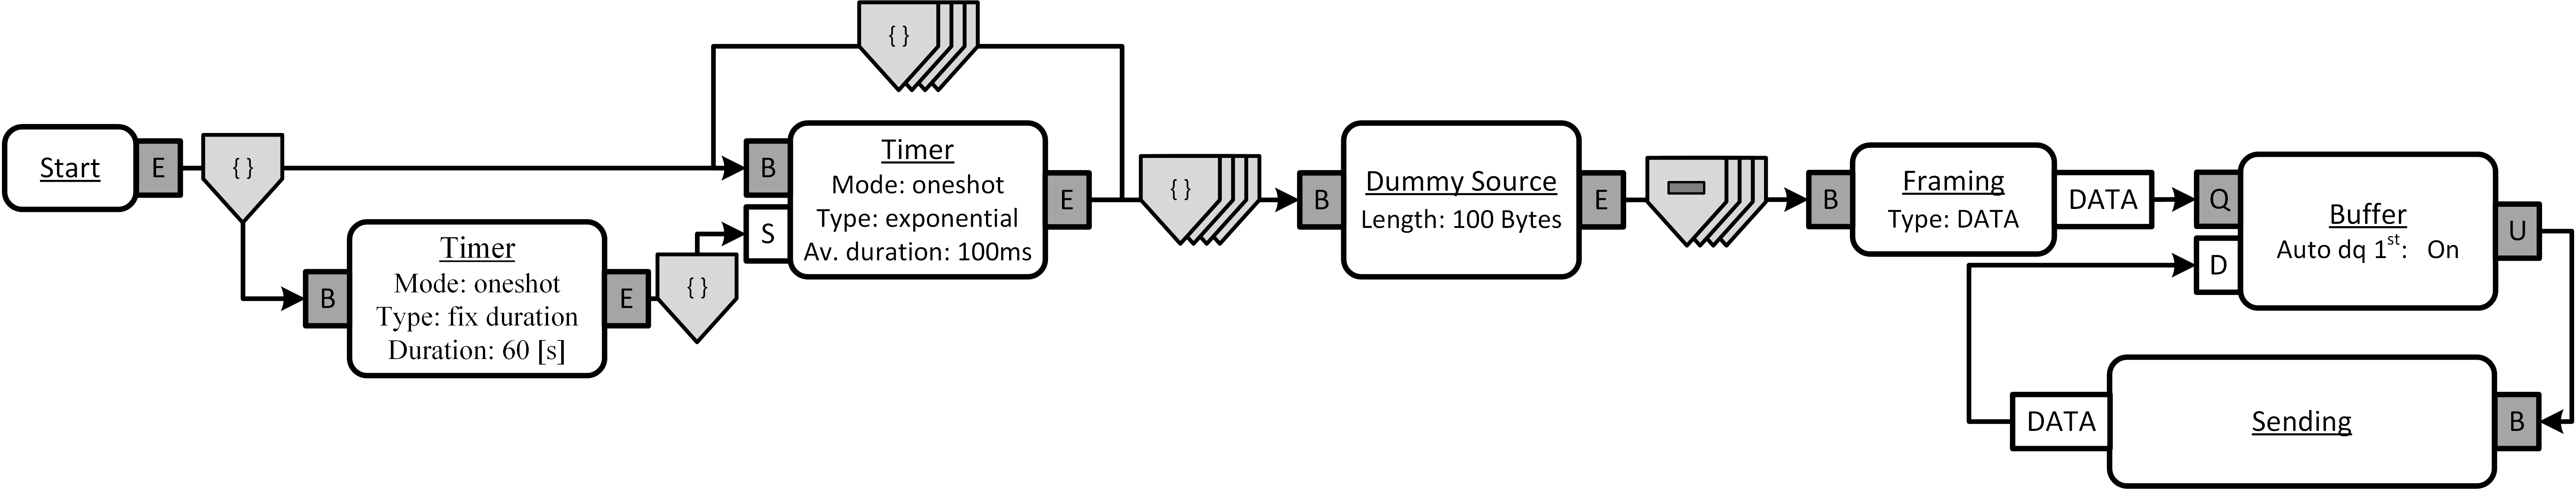
\includegraphics[width=\linewidth]{pure_aloha.png}
 		\label{fig:aloha}
	\end{figure}
\end{frame}

\begin{frame}{Where does this project fit in?}
	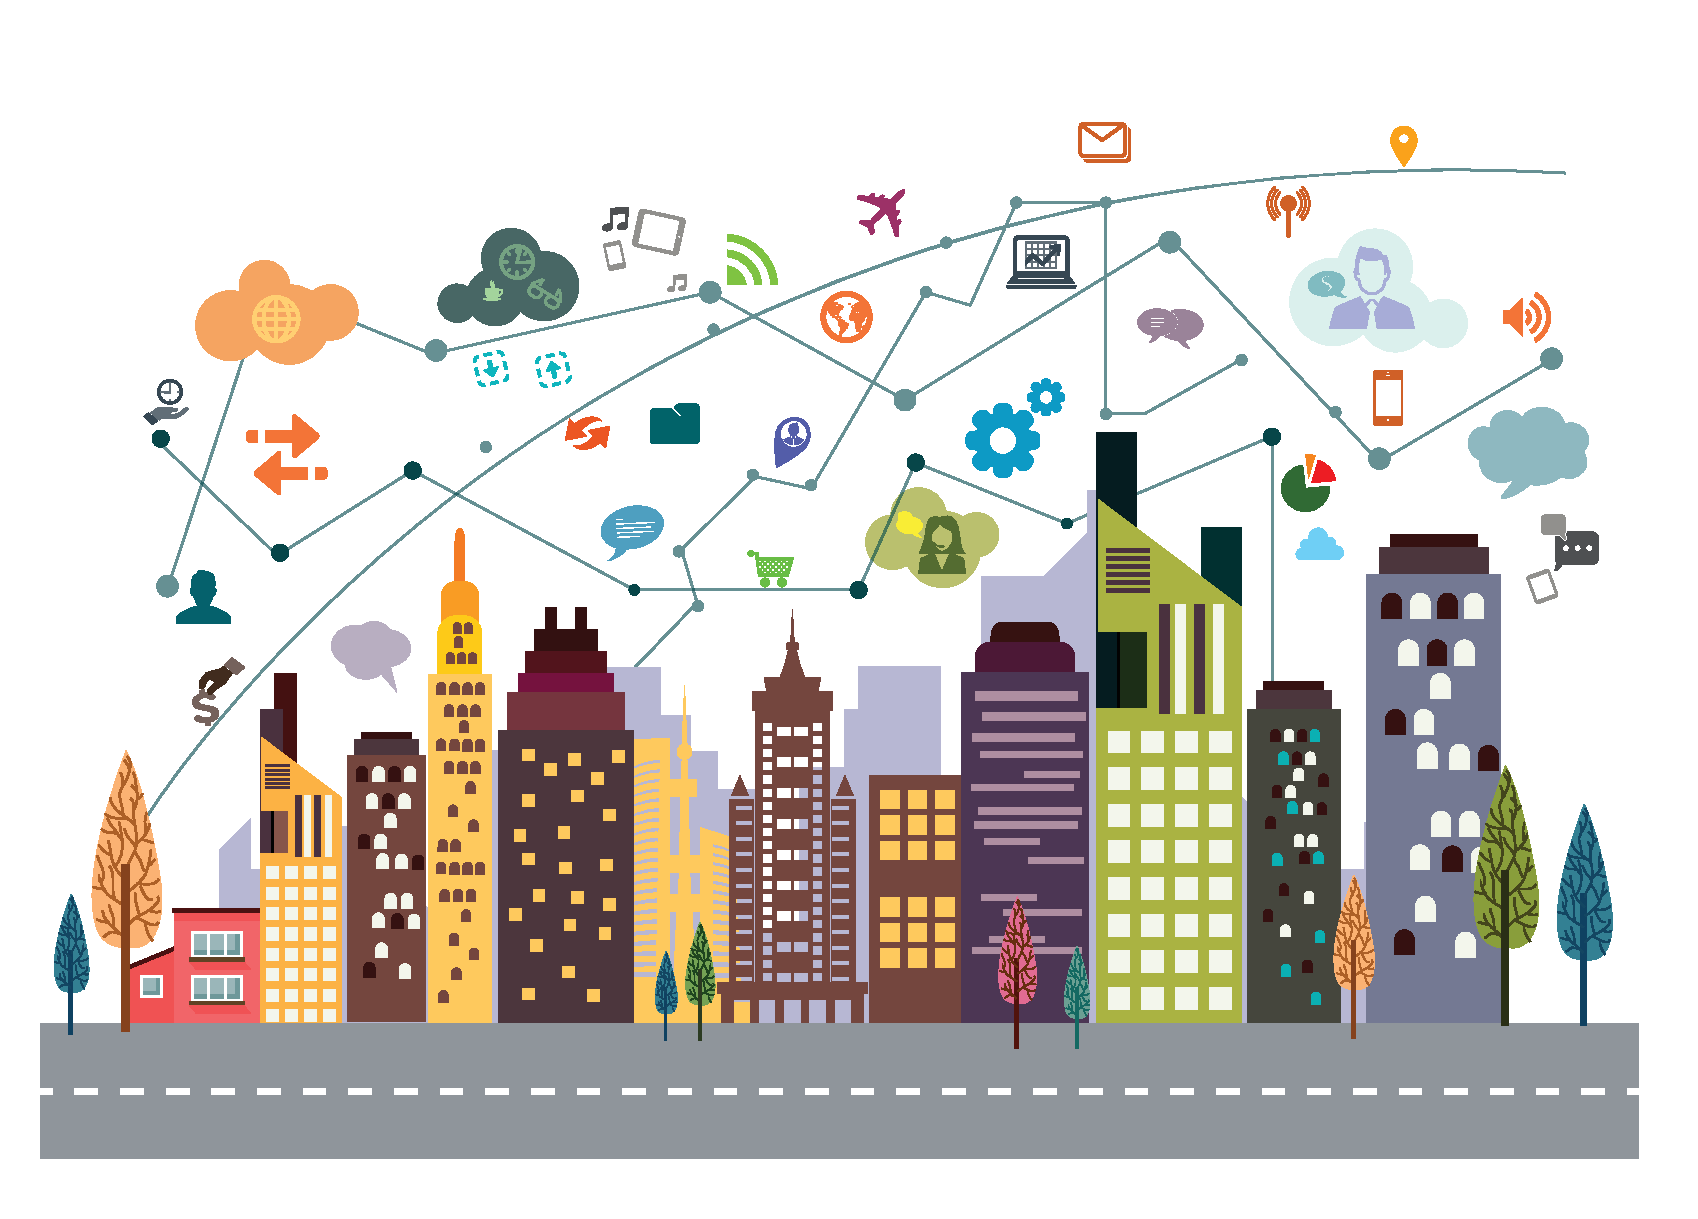
\includegraphics[width=\linewidth]{digital.eps}
	%https://all-free-download.com/free-vector/download/digital-communication-concept-cityscape-and-ui-design-style_6826344.html
\end{frame}

\section{Demo}
\begin{frame}{Demo}
Time for a quick demo!
\end{frame}

\section{Method}
\subsection{Method}
\begin{frame}{Method}
	First time doing web development \vfill
	
\includegraphics[width=0.075\linewidth]{js.png}
		%https://www.iconfinder.com/Sennerstad
	
\includegraphics[width=0.075\linewidth]{html.png}
		%By W3C, CC BY 3.0, https://commons.wikimedia.org/w/index.php?curid=12736763
 	
\includegraphics[width=0.075\linewidth]{css.png} \vfill
	Keepin' it simple \vfill
	
\includegraphics[width=0.075\linewidth]{firefox.png}
		%By The Mozilla Foundation - https://design.firefox.com/photon/visuals/product-identity-assets.htmlhttps://github.com/FirefoxUX/product-identity, CC BY 3.0,
		%https:// commons.wikimedia.org/w/index.php?curid=62823019
 	
\includegraphics[width=0.1\linewidth]{gedit.png} \vfill
		%By Henry Peters - projects.gnome.org/gedit, Commit, CC BY-SA 3.0, https://commons.wikimedia.org/w/index.php?curid=14094446
		
\end{frame}

\subsection*{Overview}
\begin{frame}{Overview}
\centering
	\begin{figure}
 		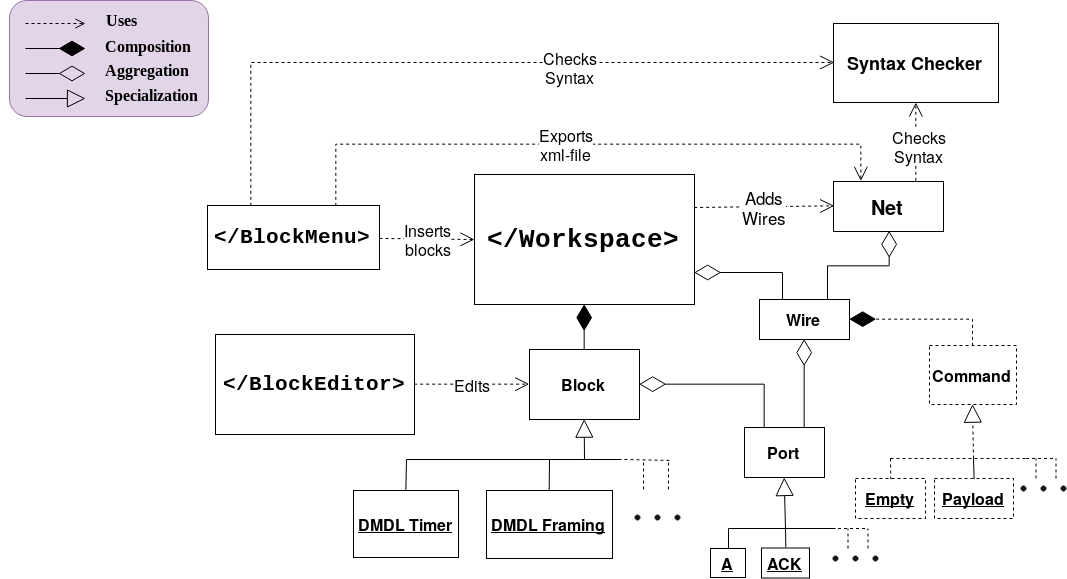
\includegraphics[width=\linewidth]{dmdl-editor.png}
		\label{fig:uml}
	\end{figure}
\end{frame}

\if 0
    \subsection{Milestones}
    \begin{frame}{Milestones}
    \centering
	    \begin{tabular}{|c|c|c|} \hline
		    \textbf{Milestone} & \textbf{Date} & \textbf{Status} \\ \hline
		    Change appearance & Nov 2nd & \color{green}{Done} \\ \hline
		    Place blocks & Nov 7th & \color{green}{Done} \\ \hline
		    Block ports & Nov 12th & \color{green}{Done} \\ \hline
		    Connect ports & Nov 19th & \color{green}{Done} \\ \hline
		    Dropdown config & Nov 29th & \color{green}{Done} \\ \hline
		    Block internals & Dec 14th & \color{red}{Partly Done} \\ \hline
		    Store config & Dec 18th & \color{red}{Done} \\ \hline
		    Check+Start buttons & Dec 21st & \color{red}{Done} \\ \hline
		    Syntax check & Jan 7th & \color{red}{Done} \\ \hline
		    Final presentation & Mid-January & \color{red}{Not Done} \\ \hline
	    \end{tabular}
    \end{frame}


    \subsection{Status}
    \begin{frame}{Status}
    \centering
	    \begin{figure}
     		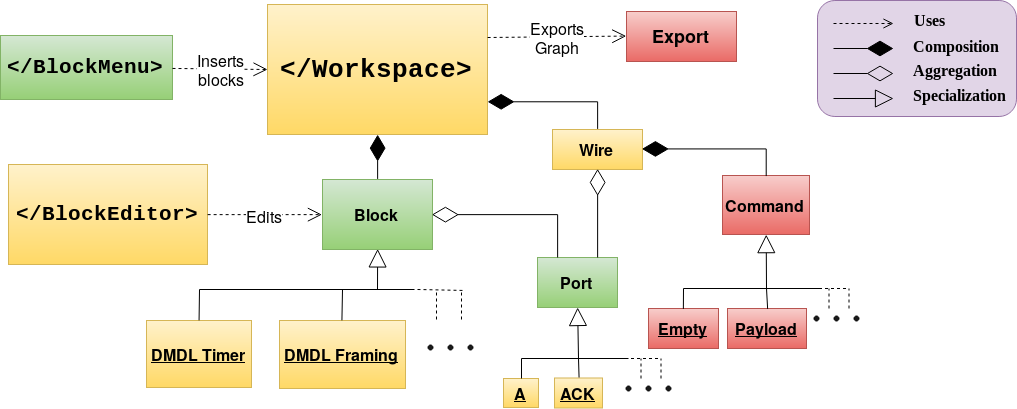
\includegraphics[width=\linewidth]{dmdl-editor-status.png}
     		\label{fig:uml-status}
	    \end{figure}
    \end{frame}
\fi

\subsection*{XML Structure}
\begin{frame}{XML Structure}
    \begin{figure}
        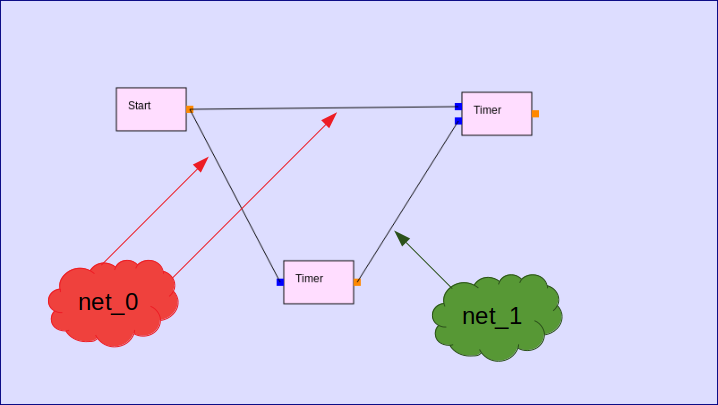
\includegraphics[width=\linewidth]{poisson_nets.png}
        \label{fig:poisson_nets}
    \end{figure}
\end{frame}
\begin{frame}{XML Structure}
    \begin{figure}
        \includegraphics[width=\linewidth]{poisson_block_cfg.pdf}
        \label{fig:poisson_block_cfg}
    \end{figure}
\end{frame}
\begin{frame}{XML Structure}
    \begin{figure}
        \includegraphics[width=\linewidth]{poisson_block_port.pdf}
        \label{fig:poisson_block_port}
    \end{figure}
\end{frame}


\subsection*{New Block Types}
\begin{frame}{New Block Types}
    \begin{figure}
        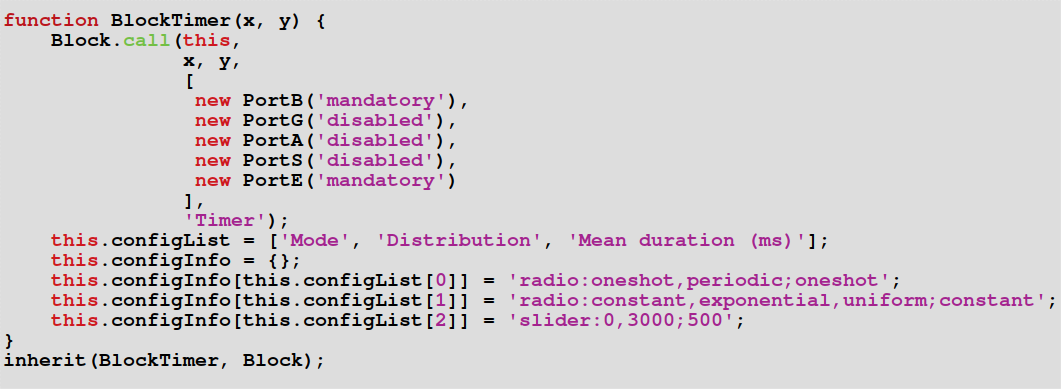
\includegraphics[width=\linewidth]{timer_src.pdf}
        \label{fig:timer_src}
    \end{figure}
\end{frame}

\section{Summary}
\begin{frame}{Summary}
	\begin{itemize}
		\item<2->  Simple drag-and-drop interface for drawing block diagrams
        \item<3->  Configurable blocks (slider, radiobutton, checkbutton)
		\item<4->  Detects loose wires
        \item<5->  Export to .xml-file for use wthin other environments
	\end{itemize}
\end{frame}

\section{Future Work}
\begin{frame}{Future Work}
	\begin{itemize}
		\item<2-> Backend that can simulate the system
		\item<3-> ''Glue'' between .xml-file and existing software
		\item<4-> Build a tool for adding new block types
	\end{itemize}
\end{frame}


\end{document}


